\documentclass[addpoints]{exam}
\usepackage{comment}            
% \begin{comment}                 
% This commented-out block of code translates default words to Spanish. 
% Remove \begin{comment} and \end{comment} to enable it.
\usepackage[spanish]{babel}
\pointpoints{punto}{puntos}
\bonuspointpoints{punto extra}{puntos extra}
\totalformat{Pregunta \thequestion: \totalpoints{} puntos}
\chqword{Pregunta}
\chpgword{Página}
\chpword{Puntos}
\chbpword{Puntos extra}
\chsword{Puntos obtenidos}
\chtword{Total}
% \end{comment}
\usepackage{datetime}
\usepackage{graphicx}
\boxedpoints
\newdate{testdate}{22}{05}{2024}

 \pagestyle{headandfoot}
 \runningheadrule
 \firstpageheader{\displaydate{testdate}}{\textbf{Escuela Politécnica Nacional}\\\textbf{Arquitectura de Computadores ICCD332-GR2}\\Prueba}{\textbf{Prof:} Lenin G. Falconí}
 \runningheader{Math 115}
 {Prueba, Página \thepage\ de \numpages}
 {\displaydate{testdate}}
 \firstpagefooter{}{}{}
 \runningfooter{}{}{}

 \begin{document}
% Quito, \displaydate{testdate} \hfill \textbf{Profesor:} Lenin
% G. Falconí M.Sc.                %
% -------------------------------------------------------------
% This code creates the text before the first question
% -------------------------------------------------------------
\begin{center}
  \fbox{\fbox{\parbox{5.5in}{ Conteste las siguientes
        preguntas en los espacios asignados. En caso de requerir más
        espacio, puede utilizar el reverso de la hoja y colocar la
        respuesta en la parte frontal}}}
\end{center}

\vspace{5mm}

\vspace{5mm}
\makebox[\textwidth]{Nombres Completos:\enspace\hrulefill}
\vspace{5mm}

% \makebox[\textwidth]{Instructor’s name:\enspace\hrulefill}


% -------------------------------------------------------------

%Here, the questions begin
\begin{questions}

%First question below
\question Convierta los siguientes números a sus equivalentes decimales.
%This question has several parts
\begin{parts}
\part[\half] $10110.0101_2$
\vspace*{\stretch{2}} %Equally distributes the available space

\part[\half] $16.5_{16}$
\vspace*{\stretch{2}}
\part[\half] $26.24_8$
\vspace*{\stretch{2}}
\end{parts}

\droptotalpoints %Prints the number of points in this question

%The next two questions are multiple choice examples
% -------------------------------------------------------------
% \question Which of these famous physicists invented time?

% \begin{oneparchoices}
%  \choice Stephen Hawking 
%  \choice Albert Einstein
%  \choice Emmy Noether
%  \choice This makes no sense
% \end{oneparchoices}

% \question Which of these famous physicists published a paper on Brownian Motion?

% \begin{checkboxes}
%  \choice Stephen Hawking 
%  \choice Albert Einstein
%  \choice Emmy Noether
%  \choice I don't know
% \end{checkboxes}
% -------------------------------------------------------------

\question Realice la operación de resta en complemento a 2. Para esto
represente los números dados en sistema binario con 8 bits.

\begin{parts}
  \part[\half] $56_{10}-63_{8}$
  \vspace*{\stretch{2}}

  \part[\half] $CC_{16}-56_{8}$
  \vspace*{\stretch{2}}

\end{parts}
\droptotalpoints %Prints the number of points in this question

\question[\half] El complemento en la base de un número $A$ en base $r$ se
define como $r^n-A$. Obtenga el complemento a 16 de AF3B

\vspace*{\stretch{2}}

\question Simplifique la siguiente expresión
$F=\bar{A}C+\bar{A}B+A\bar{B}C+BC$
\begin{parts}
  \part[\half] Usando postulados del álgebra de Boole
  \vspace*{\stretch{2}}
  \part[\half] Usando Mapa K
  \vspace*{\stretch{2}}
\end{parts}
\droptotalpoints

% \question El complemento en la base de un número $A$ en base $r$ se
% define como $r^n-A$. Obtenga:

% \begin{parts}
%   \part[\half] Complemento a 16 de AF3B
%   \vspace*{\stretch{2}}
%   \part[\half] Convierta AF3B a binario y obtenga el complemento a 2
%   \vspace*{\stretch{2}}
%   \part[\half] Convierta el resultado anterior a hexadecimal
% \end{parts}
% \droptotalpoints %Prints the number of points in this question

\clearpage

\makebox[\textwidth]{Nombres Completos:\enspace\hrulefill}
\vspace*{\stretch{2}} \question[2] Exprese en formato IEEE de 32 bits el número
$-48.75$. Escriba el resultado en notación hexadecimal. %\answerline

\vspace*{\stretch{2}}


\question[2] Obtenga el valor decimal equivalente del número expresado en
formato  IEEE de 32 bits: $C3C00000$. %\answerline

\vspace*{\stretch{2}}


\question[2] La Figura \ref{fig:circuito} muestra un diagrama de un
circuito para la alarma de un automóvil. Los 3 sensores, representados
como interruptores, indican el estado de la puerta del conductor
$S_p$, el interruptor de encendido del coche $I$ y las luces frontales
$S_l$, respectivamente. Diseñe un circuito lógico
simplificado\footnote{Obtenga la tabla de verdad y simplifique usando
  Mapas K} con estos tres interruptores como
entradas de manera que la alarma se active cuando exista cualquiera de
las siguientes condiciones:

\begin{itemize}
  \item Las luces frontales están prendidas, mientras el interruptor del
  encendido está apagado.
\item La puerta está abierta mientras el interruptor de encendido está
  activado
\end{itemize}


\begin{figure}[h!]
  \centering
  \caption{Circuito de Alarma de Vehículo}
  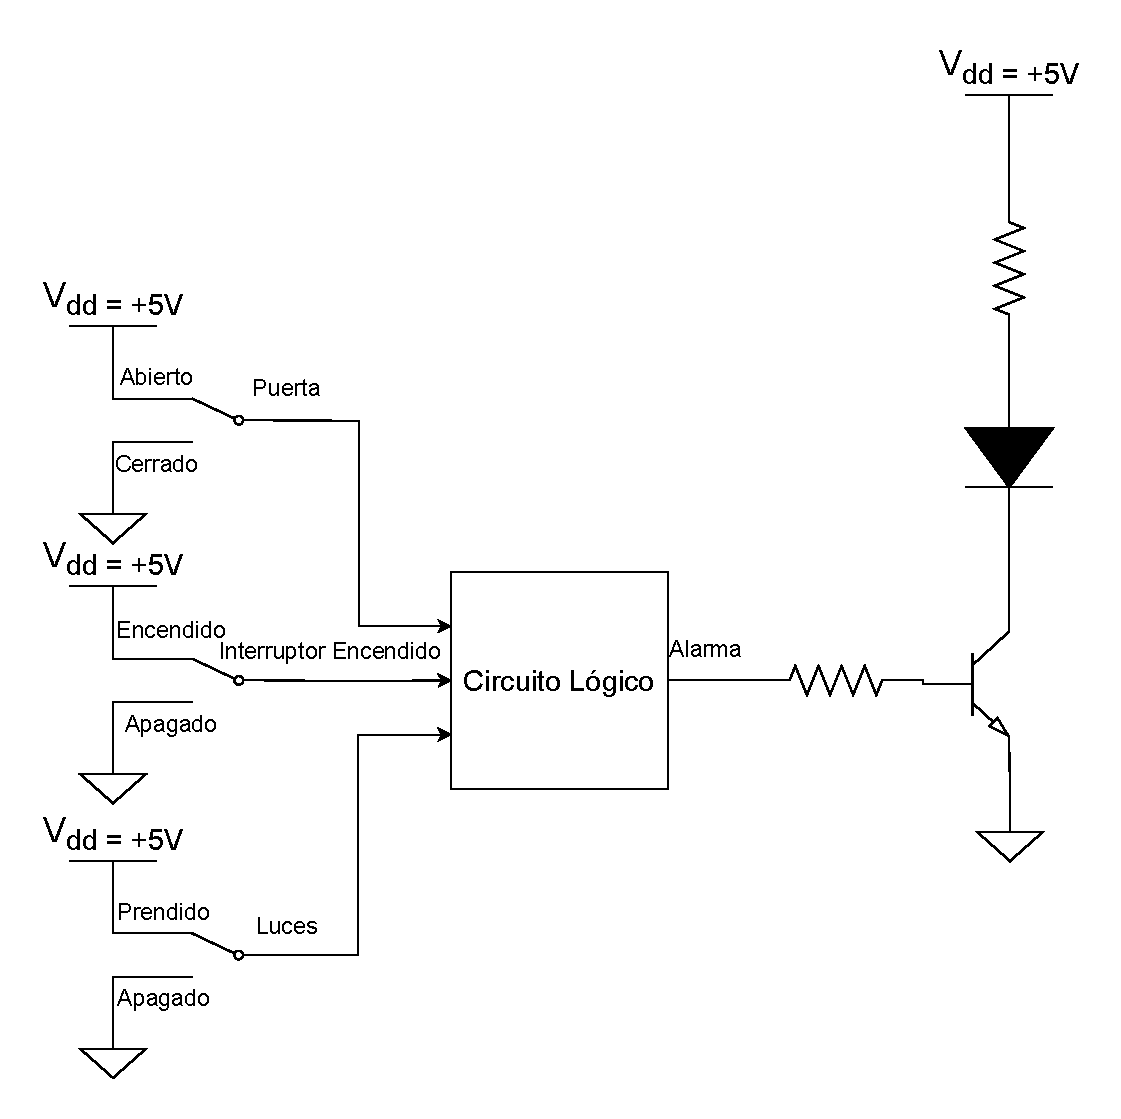
\includegraphics[scale=0.6]{./images/Problema4-8.pdf}
  \label{fig:circuito}
\end{figure}


\end{questions}

\begin{center}
  \scriptsize
  \combinedgradetable[h][questions]
\end{center}

\end{document}
